\thispagestyle{lichsutoanhocnone}
\pagestyle{lichsutoanhoc}
\graphicspath{{../lichsutoanhoc/pic/}}
\everymath{\color{lichsutoanhoc}}
\blfootnote{$^1$\color{lichsutoanhoc}Cộng tác viên Viện Toán học.}
\begingroup
\AddToShipoutPicture*{\put(0,616){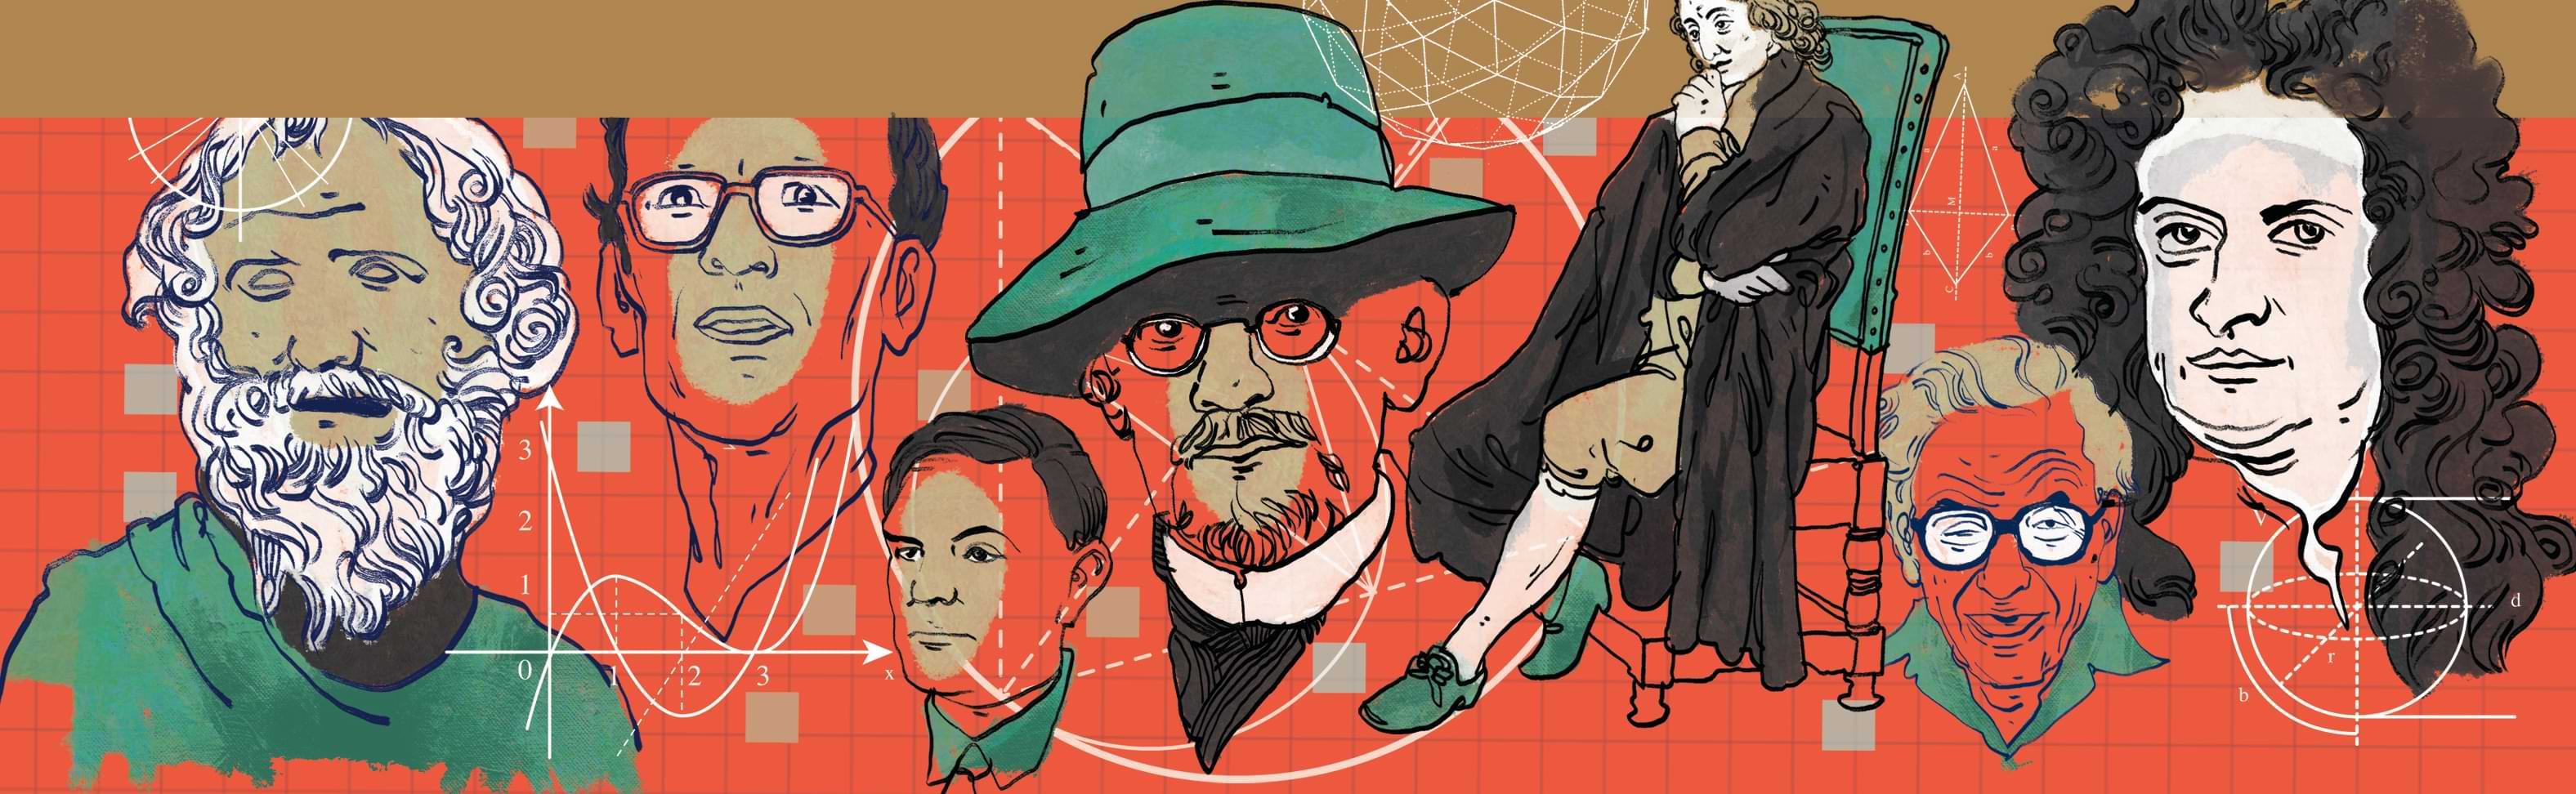
\includegraphics[width=19.3cm]{../bannerlichsu}}}
\AddToShipoutPicture*{\put(100,525){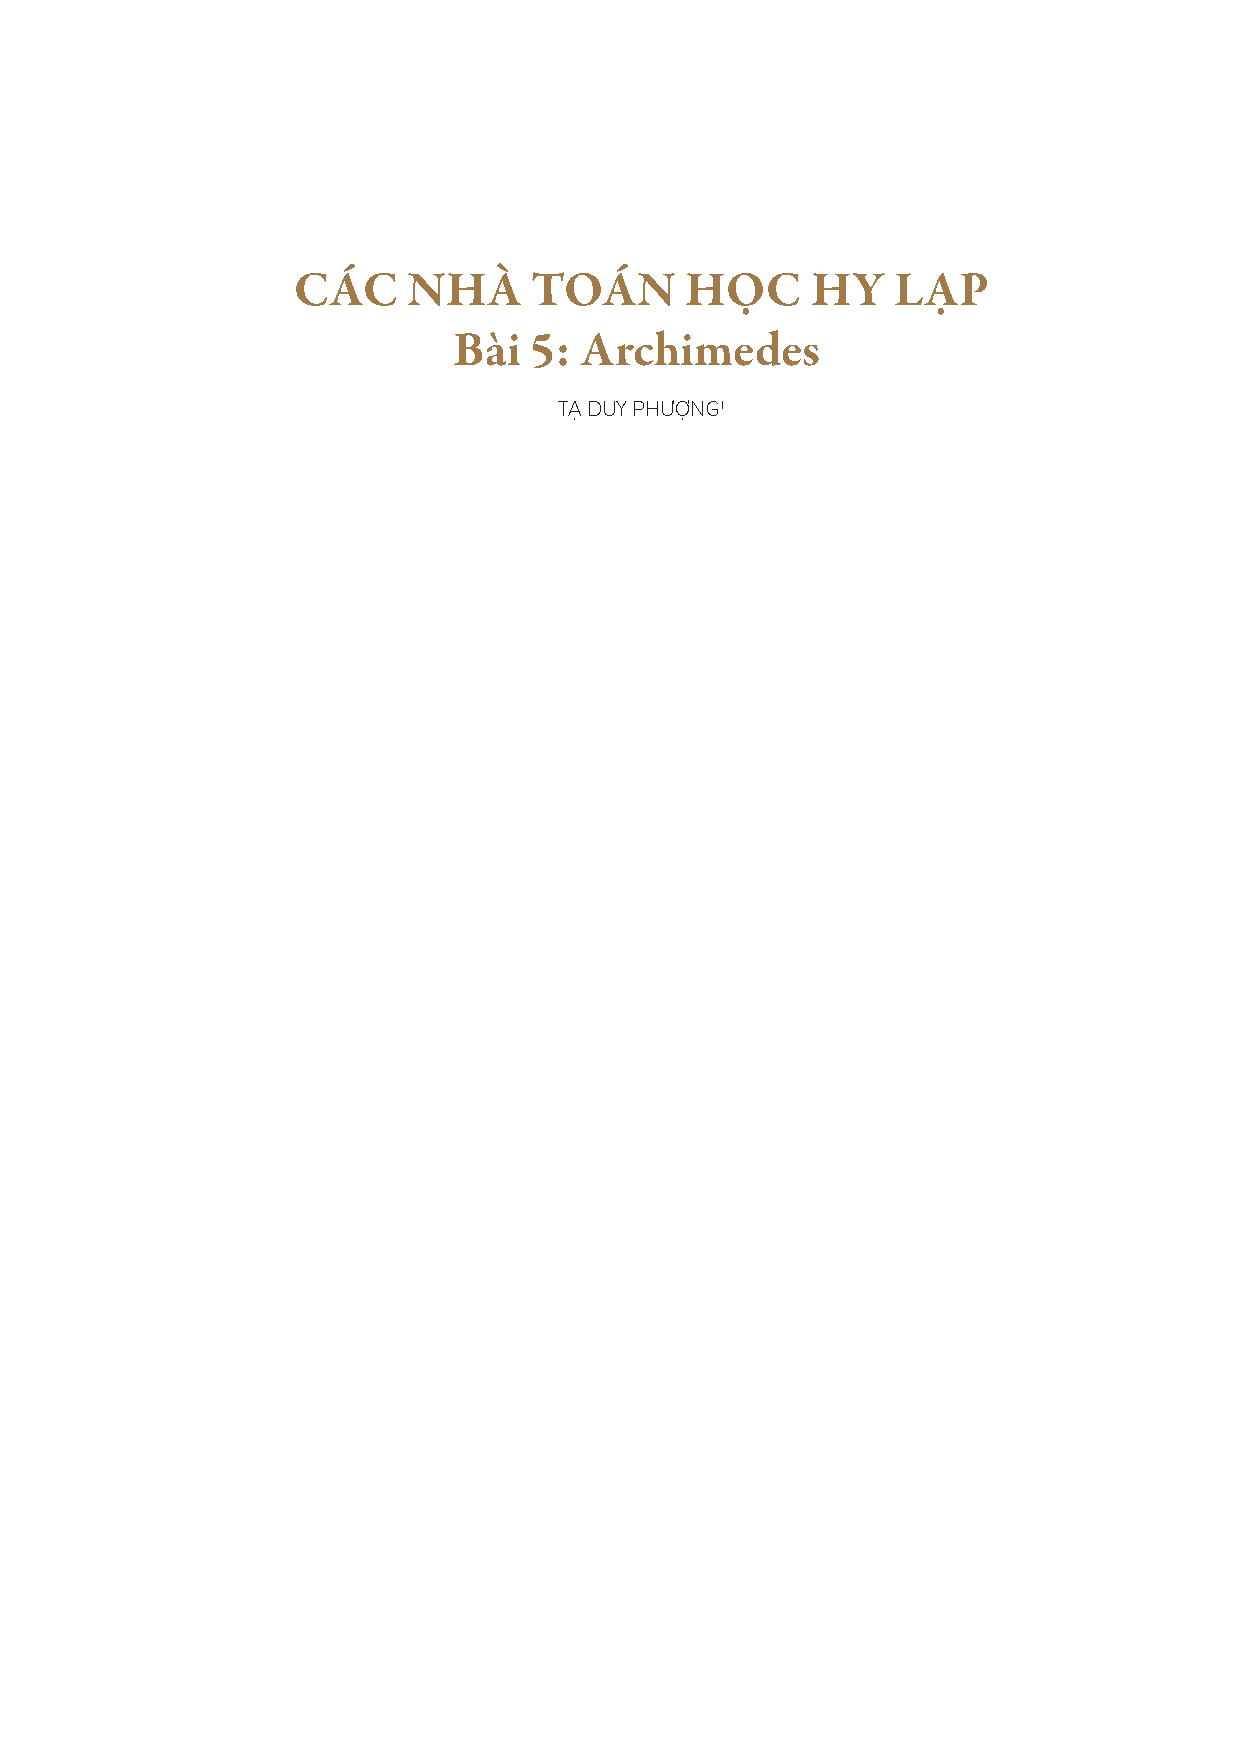
\includegraphics[scale=1]{../tieude.pdf}}}
\centering
\endgroup

\vspace*{182pt}

\begin{multicols}{2}
	\begin{figure}[H]
		\vspace*{5pt}
		\centering
		\captionsetup{labelformat= empty, justification=centering}
		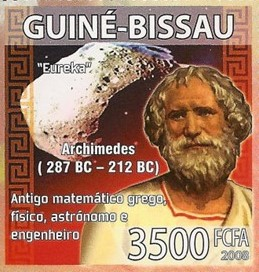
\includegraphics[width= 1\linewidth]{1}
		%		\caption{\small\textit{\color{}.}}
		\vspace*{-20pt}
	\end{figure}
	\textbf{\color{lichsutoanhoc}Nhập đề.} Archimedes ($287-212$ trước CN) sống mãi với nhân loại bởi những những công trình toán học, những cống hiến của ông trong kỹ thuật và trong công cuộc bảo vệ đất nước, và còn bởi những huyền thoại về ông (xem, thí dụ, [$9$]).
	\vskip 0.1cm
	Ông là con trai của Phidias, một nhà thiên văn học, người bà con và người bạn của vua Hieron II xứ Syracuse. Vì vậy, Archimedes đã được vua Hieron II cấp học bổng đi du học ở Alexandria (trung tâm khoa học và văn hóa thời bấy giờ) từ năm $11$ tuổi. Tại Alexandria, ông đã nghiên cứu toán học với những học trò của Euclid. Ông có quan hệ thân thiết với các nhà toán học nổi tiếng và có thói quen thông báo những khám phá toán học của mình cho Eratosthenes và những người khác trước khi chúng được phổ biến rộng rãi.  
	\vskip 0.1cm
	Sau khi trở về Syracuse, ông dành toàn bộ cuộc đời mình cống hiến cho toán học. 
	\vskip 0.1cm
	Bài viết này giới thiệu đôi nét \textit{Con người và Sự nghiệp} của Archimedes, những đóng góp trong toán học, vị trí của ông trong toán học Hy Lạp và toán học hiện đại qua các tác phẩm ông để lại. 
	\begin{figure}[H]
		\vspace*{-5pt}
		\centering
		\captionsetup{labelformat= empty, justification=centering}
		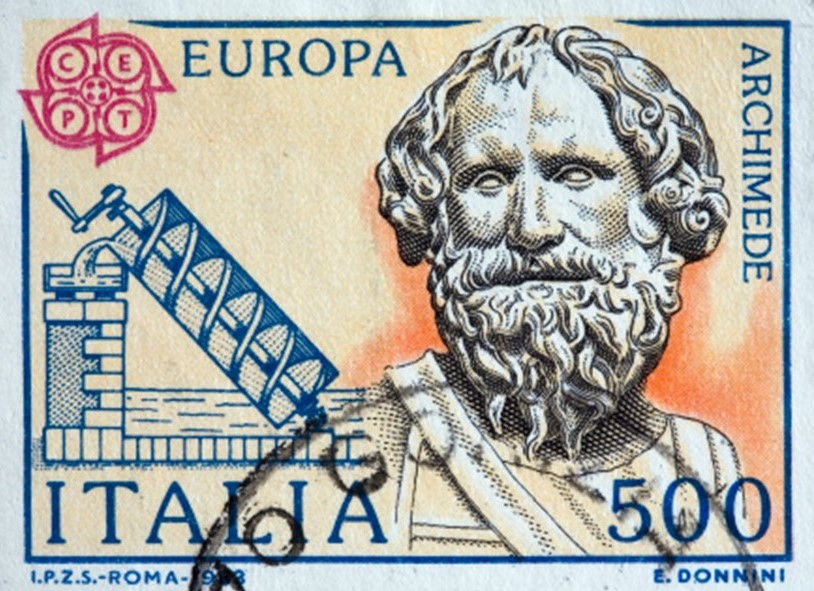
\includegraphics[width= 1\linewidth]{2}
		\caption{\small\textit{\color{lichsutoanhoc}Archimedes và bơm xoắn trên tem của Italia. Có thể tìm hiểu nguyên lý vận hành của bơm xoắn Archimedes qua các video trên mạng internet.}}
		\vspace*{-10pt}
	\end{figure}
	\textbf{\color{lichsutoanhoc}Những tác phẩm và thành tựu khoa học của Archimedes.} Khi học ở Alexandria, Archimedes đã chế tạo ra \textit{bơm xoắn} hay \textit{bơm trục vít} (water--screw hay screw pump), sau này mang tên bơm xoắn Archimedes, giải quyết vấn đề thời sự của xã hội lúc bấy giờ là nhu cầu bơm nước từ dưới sông Nile lên tưới ruộng. Ngày nay, nguyên lý vận hành của bơm xoắn Archimedes vẫn được ứng dụng trong tất cả các máy bơm có trục xoắn. 
	\begin{figure}[H]
		\vspace*{-5pt}
		\centering
		\captionsetup{labelformat= empty, justification=centering}
		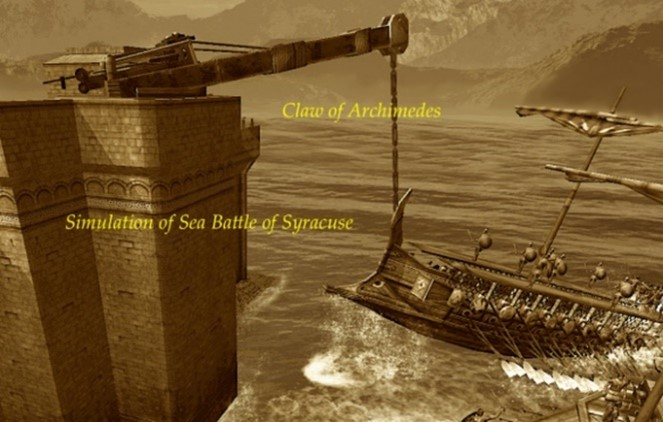
\includegraphics[width= 1\linewidth]{3}
		\caption{\small\textit{\color{lichsutoanhoc}Móng thép Archimedes được sử dụng trong chiến tranh chống quân xâm lược La Mã.}}
		\vspace*{-10pt}
	\end{figure}
	Trong công cuộc bảo vệ thành phố quê hương Syracuse trước sự xâm lược của quân đội La Mã, Archimedes đã chế tạo ra rất nhiều máy móc (súng bắn đá, ròng rọc, cần cẩu,\ldots) phục vụ cho quân đội. Những máy móc này đã làm kinh hoàng lính La Mã đến mức khi nhìn thấy một đoạn dây thừng hoặc một cây gỗ nhô ra phía trên bức tường thành, họ đã khóc và thét lên: ``Nó đấy!" và tưởng tượng ra Archimedes đang khởi động một động cơ nào đó chống lại họ, và quay lưng bỏ chạy.
	\begin{figure}[H]
		\vspace*{-5pt}
		\centering
		\captionsetup{labelformat= empty, justification=centering}
		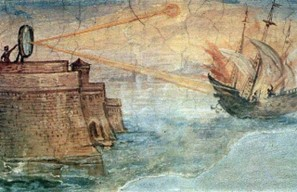
\includegraphics[width= 1\linewidth]{4}
		\caption{\small\textit{\color{lichsutoanhoc}Hệ thống gương lõm đốt cháy tàu. 
				Ảnh minh họa: Wearethemighty}}
		\vspace*{-5pt}
	\end{figure}
	Câu chuyện về Archimedes đốt cháy các con tàu La Mã bằng cách sắp xếp các gương lõm được tìm thấy trong tác phẩm của Lucian ($125-180$ Công nguyên). Tuy nhiên, sau nhiều thí nghiệm thành công được thực hiện nghiêm túc vào thế kỷ XX, người ta vẫn nghi ngờ câu chuyện này, vì vũ khí này quá phức tạp, quá tốn kém và ít hiệu quả (phụ thuộc thời tiết,\ldots) so với các vũ khí khác (thí dụ, mũi tên tẩm dầu lửa, súng phun lửa,\ldots). 
	\begin{figure}[H]
		\vspace*{-5pt}
		\centering
		\captionsetup{labelformat= empty, justification=centering}
		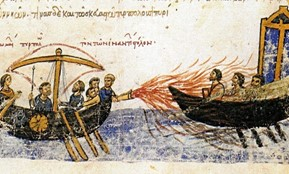
\includegraphics[width= 1\linewidth]{5}
		\caption{\small\textit{\color{lichsutoanhoc}Súng phun lửa. Ảnh minh họa: Wearethemighty.}}
		\vspace*{-10pt}
	\end{figure}
	\textbf{\color{lichsutoanhoc}Toán học của Archimedes.} Archimedes thường được biết đến như là nhà phát minh các thiết bị cơ khí với sự sáng tạo tài tình, hơn là những phát minh toán học lý thuyết. Nhưng hơn ai hết, ông là nhà toán học vĩ đại, có thể là vĩ đại nhất mọi thời đại, và là người đầu tiên biết ứng dụng toán học lý thuyết ở trình độ cao vào giải quyết các bài toán nảy sinh từ thực tế, đồng thời, các bài toán thực tế cũng giúp Archimedes phát minh ra những lý thuyết toán học mới (thủy tĩnh học,\ldots).
	\vskip 0.1cm 
	Một số tác phẩm của Archimedes với những lời bình luận sâu sắc của Eutocius vào đầu thế kỷ VI đã được tìm thấy trong một ấn phẩm ở gần Byzantium. Ấn bản này là cơ sở của một số phần trong ba bộ sưu tập các tác phẩm của Archimedes được viết trên giấy da, đã từng tồn tại ở Byzantium vào thế kỷ X--XI. Năm $1906$, J. L. Heiberg, người biên tập các văn bản của Archimedes, đã giải mã và công bố nội dung toán học trên một tấm da cừu tìm thấy trong thư viện Jerusalem tại Constantinople. Điều này chứng tỏ rằng các tác phẩm của Archimedes đã được phổ biến, lưu truyền qua các bản chép tay từ trước thế kỷ thứ X. Bản thảo lâu đời thứ hai còn tồn tại là bản dịch tiếng Latin năm $1260$, có lẽ là hợp của hai bản dịch từ bản Byzantium đã bị mất. Ngoài ra, còn một số bản sao Hy Lạp thế kỷ XV--XVI của các phiên bản Byzantium bị thiếu. Heiberg đã đối chiếu những bản thảo này và đã tạo ra văn bản của Archimedes bằng tiếng Hy Lạp tiêu chuẩn hiện nay vào năm $1880-1881$, với một phiên bản sửa đổi năm $1910$. Tuy nhiên, nếu như  \textit{Cơ sở} (Elements) của Euclid được phổ biến rộng rãi, thì các tác phẩm của Archimedes chỉ được lưu truyền trong nhóm nhỏ các nhà toán học lỗi lạc nhất của thời đại ông và sau này. Các tác phẩm của Archimedes hiện được tìm thấy gồm:
	\vskip 0.1cm
	$1.$ Về hình cầu và hình trụ (On the Sphere and Cylinder, hai quyển);
	\vskip 0.1cm
	$2.$ Phép đo hình tròn (Measurement of a Circle); 
	\vskip 0.1cm
	$3.$ Về hình nón và hình cầu (On Conoids and Spheroids); 
	\vskip 0.1cm
	$4.$ Về đường xoắn ốc (On Spiral);
	\vskip 0.1cm
	$5.$ Cân bằng phẳng (On Plane Equilibriums, hai quyển);
	\vskip 0.1cm
	$6.$ Người tính cát (The Sand--reckoner);
	\vskip 0.1cm
	$7.$ Cầu phương Parabola (Quadrature of the Parabola);
	\vskip 0.1cm
	$8.$ Về vật nổi (On floating Bodies, hai quyển); 
	\vskip 0.1cm
	$9.$ Sách về các bổ đề (Book of Lemmas);
	\vskip 0.1cm
	$10.$~Bài toán về gia súc (The Cattle--Problem). 
	\vskip 0.1cm
	$11.$ Phương pháp (The Method).
	\vskip 0.1cm
	Ngoài ra, còn một số tác phẩm bị thất lạc.
	\vskip 0.1cm
	Một tỷ lệ lớn bất thường các chủ đề trong các tác phẩm của Archimedes đại diện cho các khám phá hoàn toàn mới của riêng ông. Mặc dù các nghiên cứu của ông có nội dung rộng lớn gần như bách khoa toàn thư, bao gồm hình học (phẳng và không gian), số học, cơ học, thủy tĩnh học, nhưng ông không phải là người viết sách giáo khoa. Tác phẩm của Archimedes, giống như tác phẩm của Euclid trước ông, phần lớn bao gồm hệ thống hóa, khái quát hóa các phương pháp đã được sử dụng và các kết quả riêng lẻ của các nhà hình học trước đó. Archimedes không chỉ gia công những vật liệu hiện có, mà mục tiêu của ông luôn là một cái gì đó mới, một số bổ sung nhất định và độc đáo cho kiến thức tổng thể. 
	\vskip 0.1cm
	Đặc điểm nổi bật của con người Archimedes là sự bộc trực và đơn giản, hoàn toàn không có chủ nghĩa vị kỉ và bất kì nỗ lực nào phóng đại thành tích của mình bằng cách so sánh với thành tích của những người khác hoặc nhấn mạnh những thất bại của họ ở những nơi mà bản thân ông đã thành công. Cách của ông chỉ đơn giản là nêu những khám phá cụ thể mà những người tiền nhiệm thực hiện đã gợi ý cho ông về khả năng mở rộng chúng theo hướng mới. Thí dụ, liên quan đến những nỗ lực của các nhà hình học trước đó nhằm cầu phương hình tròn và các hình khác, Archimedes chợt nhận ra rằng chưa có ai từng cầu phương parabola, ông đã đặt và giải quyết trọn vẹn bài toán này. Tương tự, trong lời nói đầu của cuốn sách \textit{Về hình cầu và hình trụ}, ông nói về những khám phá của mình liên quan đến những hình khối như các định lý về hình chóp, hình nón và hình trụ đã được chứng minh bởi Eudoxus.  ông không ngần ngại nói rằng một số vấn đề đã làm ông mất nhiều năm mới giải quyết được. Trong lời nói đầu của cuốn sách \textit{Về đường xoắn ốc}, ông khẳng định, nếu không vì cái chết đột ngột, Conon đã giải được các bài toán mà ông trình bày. 
	\vskip 0.1cm
	Trong một số chủ đề, Archimedes không có người đi trước. Thí dụ trong thủy tĩnh học, nơi ông đã phát minh ra toàn bộ khoa học này, và vì vậy, những phát minh toán học liên quan đến chúng. Trong những lĩnh vực này, ông là người đặt nền móng cho một bộ môn khoa học mới. Và ông trình bày bắt đầu gần giống như sách giáo khoa tiểu học, nhưng ở các phần sau, ngay lập tức, ông đã trình bày các nghiên cứu chuyên sâu. 
	\vskip 0.1cm
	Để thấy rõ những phát minh của Archimedes, cần tham chiếu với một số thành tựu khoa học đã đạt được trước ông.
	\vskip 0.1cm
	\textbf{\color{lichsutoanhoc}Các phương pháp hình học truyền thống.} \textit{Đại số hình học} (geometrical algebra) đã đóng vai trò quan trọng trong hình học Hy Lạp. Hai phương pháp chính bao gồm trong thuật ngữ này là: ($1$) Lý thuyết về tỷ lệ (theory of proportions); ($2$) Phương pháp diện tích. Cả hai phương pháp này đều đã được trình bày đầy đủ trong \textit{Cơ sở} của Euclid. Đại số hình học cũng đã được Archimedes sử dụng hiệu quả. 
	\vskip 0.1cm
	\textbf{\color{lichsutoanhoc}Phép cầu phương và lập phương.} Hai định lý mà Archimedes gán cho Eudoxus là:
	\vskip 0.1cm
	($1$) \textit{Mọi lăng trụ có thể tích bằng ba lần thể tích hình chóp có cùng đáy và chiều cao.} 
	\vskip 0.1cm
	Gọi  $V_1$ và $V_2$ tương ứng là thể tích hình lăng trụ và thể tích hình chóp có cùng diện tích đáy là $S$  và chiều cao $h$. Khi đó:
	\begin{align*}
		V_1 = Sh = 3\times\frac{1}{3}Sh = 3V_2.
	\end{align*}
	($2$) \textit{Mọi hình trụ có thể tích bằng ba lần thể tích hình nón có cùng đáy và chiều cao.}
	\vskip 0.1cm
	Các Mệnh đề dưới đây cũng được Archimedes cho là của các tác giả trước:  
	\vskip 0.1cm
	($3$) \textit{Các hình nón có chiều cao bằng nhau thì tỷ số thể tích của chúng bằng tỷ số diện tích đáy.}
	\vskip 0.1cm
	($4$) \textit{Nếu một hình trụ bị chia bởi một mặt phẳng song song với đáy thì tỷ số thể tích của hai hình trụ bị chia bằng tỷ số hai đường cao của chúng.}
	\vskip 0.1cm
	($5$) \textit{Nếu hai hình nón có đáy và chiều cao bằng đáy và chiều cao của hai hình trụ tương ứng thì tỷ số thể tích của hai hình nón bằng tỷ số thể tích của hai hình trụ đó.}
	\vskip 0.1cm
	($6$) \textit{Tỷ số diện tích đáy của hai hình nón có thể tích bằng nhau tỷ lệ nghịch với tỷ số chiều cao của chúng và ngược lại. }
	\vskip 0.1cm
	($7$) \textit{Hai hình nón có tỷ số đường kính bằng tỷ số đường cao thì tỷ số thể tích của chúng bằng lũy thừa bậc ba của tỷ số ấy.} 
	\vskip 0.1cm
	Trong cuốn \textit{Cầu phương Parabola}, Archimedes cũng nói rằng các nhà hình học trước đã chứng minh:
	\vskip 0.1cm
	($8$) \textit{Tỷ số thể tích hình cầu bằng lũy thừa bậc ba tỷ số đường kính của chúng.}
	\vskip 0.1cm
	Trong tất cả các tác phẩm của mình, có vẻ như Archimedes tự hào nhất về cuốn chuyên luận \textit{Về hình cầu và hình trụ}. Tác phẩm được viết thành hai quyển. Quyển I gồm $44$ mệnh đề ([$2$], trang $141-187$; [$3a$], trang $1-55$). Cuốn sách mở đầu bằng thông báo các kết quả do chính ông nhận được và lần đầu tiên được xuất bản \textit{để các nhà toán học lão luyện có thể kiểm tra tính chính xác và đánh giá giá trị của chúng}. Hai mệnh đề được nói đến trong lời mở đầu là:
	\vskip 0.1cm
	($1$) \textit{Diện tích mặt cầu bằng $4$ lần diện tích hình tròn lớn nhất của mặt cầu}.
	\vskip 0.1cm
	Theo ngôn ngữ hiện đại: $S_1 = 4\pi R^2$.
	\vskip 0.1cm
	($2$) \textit{Nếu hình trụ ngoại tiếp hình cầu có chiều cao bằng đường kính hình cầu thì thể tích của nó bằng $\frac{3}{2}$ thể tích hình cầu; Và diện tích toàn phần hình trụ bằng $\frac{3}{2}$ diện tích mặt cầu.}  
	\begin{figure}[H]
		\vspace*{-5pt}
		\centering
		\captionsetup{labelformat= empty, justification=centering}
		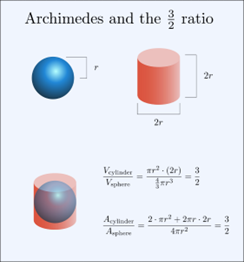
\includegraphics[width= 0.8\linewidth]{6}
%		\caption{\small\textit{\color{}.}}
		\vspace*{-10pt}
	\end{figure}
	Công thức tính thể tích hình cầu:  ${V_1} = \frac{4}{3}\pi {R^3}$.
	\vskip 0.1cm
	Thể tích hình trụ: 
	\begin{align*}
		{V_2} = {S_d} \times h = \pi {R^2} \times h = 2\pi {R^3} = \frac{3}{2}{V_1}.
	\end{align*}
	Diện tích toàn phần hình trụ: 
	\begin{align*}
		{S_2} &= 2{S_d} + {S_{xq}} = 2\pi {R^2} + 2\pi R\times2R \\
		&= 6\pi {R^2} = \frac{3}{2}{S_1}.
	\end{align*}
	Tiếp theo là một số định nghĩa và giả định (assumptions) hay tiên đề. Một tiên đề nổi tiếng nhất mà ngày nay được gọi là \textit{Tiên đề} hay \textit{Định đề Archimedes}, trong khi chính Archimedes lại gán định đề này cho Eudoxus, là:  
	\vskip 0.1cm
	\textit{Hai đoạn thẳng không bằng nhau thì bội của cái ngắn hơn sẽ vượt quá cái dài hơn.}
	\vskip 0.1cm 
	Sử dụng định đề này, Archimedes đã rút ra nhiều kết quả liên quan đến diện tích hoặc thể tích hình giới hạn bởi đường cong hoặc mặt cong.
	\vskip 0.1cm
	Quyển II của \textit{Về hình cầu và hình trụ} gồm $6$ mệnh đề, thực chất là $6$ bài toán, và $3$ định lý ([$2$], trang $187-221$; [$3a$], trang $56-90$) được gợi ý bởi Quyển I. Khi giải quyết bài toán về thiết diện của hình cầu, Archimedes (Mệnh đề $4$, Quyển II) đã đặt ra một trong những bài toán lớn của hình học Hy Lạp: 
	\vskip 0.1cm
	\textit{Dựng mặt phẳng cắt mặt cầu sao cho thể tích hai phần mặt cầu bị chia theo một tỷ lệ $\frac{m}{n}$ cho trước.} 
	\vskip 0.1cm
	Bài toán này có thể hiểu như sau: Gọi bán kính hình cầu là $R$  và chiều cao của hai chỏm cầu bị chia là $h$  và $h'$  ($h+ h'= 2R$). Vì thể tích chỏm cầu chiều cao $h$ là $V = \pi {h^2}\left( {R - \frac{h}{3}} \right)$  nên 
	\begin{align*}
		\frac{m}{n} = \frac{V}{{V'}} = \frac{{\pi {h^2}\left( {R - \frac{h}{3}} \right)}}{{\pi {{h'}^2}\left( {R - \frac{{h'}}{3}} \right)}} = \frac{{{h^2}\left( {3R - h} \right)}}{{{{h'}^2}\left( {3R - h'} \right)}}.
	\end{align*}
	Thay $h' = 2R - h$  vào phương trình trên ta được
	\begin{align*}
		m{\left( {2R - h} \right)^2}\left( {R + h} \right) = n{h^2}\left( {3R - h} \right).
	\end{align*}
	Hay 
	\begin{align*}
		\left( {m \!+\! n} \right){h^3} \!-\! 3R\left( {m \!+\! n} \right){h^2} \!+\! 4m{R^3} \!=\! 0. \tag{$*$}
	\end{align*}
	Bài toán $4.$ II có nhiều tiếp cận hình học (xem, [$8$], trang $172-185$; [$4$], trang $44-49$) và dẫn đến việc giải phương trình bậc ba ($*$). Phương trình bậc ba tổng quát chỉ được giải trọn vẹn hơn nghìn năm sau bởi các nhà toán học châu Âu.
	\vskip 0.1cm
	Trong số các tác phẩm của Archimedes được biết đến trong thời Trung cổ, phổ biến nhất và là tác phẩm đầu tiên được dịch sang tiếng Latin là \textit{Phép đo hình tròn}. Đây là một chuyên luận ngắn ([$2$], trang $222-239$; [$3a$], trang $91-98$), có lẽ là một phần của một tác phẩm dài hơn đã bị thất lạc, chỉ bao gồm ba mệnh đề. 
	\vskip 0.1cm
	Mệnh đề $1$ nói rằng diện tích của hình tròn có thể tính theo chu vi của nó:
	\vskip 0.1cm
	\textbf{\color{lichsutoanhoc}Mệnh đề} $\pmb{1.}$ \textit{Diện tích của bất kì hình tròn nào cũng bằng diện tích của tam giác vuông có một cạnh góc vuông bằng bán kính và cạnh góc vuông kia bằng chu vi đường tròn.}
	\vskip 0.1cm
	Theo ngôn ngữ hiện đại: $S = \frac{1}{2}R \times 2\pi R = \pi {R^2}.$
	\vskip 0.1cm 
	Mệnh đề $2$ cho đánh giá xấp xỉ diện tích hình tròn:
	\vskip 0.1cm
	\textbf{\color{lichsutoanhoc}Mệnh đề} $\pmb{2.}$ \textit{Tỷ lệ diện tích hình tròn với diện tích hình vuông ngoại tiếp nó rất gần bằng $11:14$}.
	\vskip 0.1cm
	Mệnh đề $3$ là mệnh đề quan trọng nhất trong \textit{Phép đo hình tròn}.
	\vskip 0.1cm
	\textbf{\color{lichsutoanhoc}Mệnh đề} $\pmb{3.}$ \textit{Chu vi của mọi đường tròn không vượt quá $3\frac{1}{7}$ và lớn hơn $3\frac{10}{71}$  đường kính của nó.}
	\vskip 0.1cm
	Từ đây ta có: 
	\begin{align*}
		3{,}140845... &\approx 3\frac{{10}}{{71}} < \pi  \approx 3{,}14159 < 3\frac{1}{7} \\
		&\approx 3{,}142857.
	\end{align*}
	Đo hình tròn đã được trình bày tỷ mỉ trong tạp chí Pi, [$10$], [$12$], [$13$], vì vậy ở đây không nhắc lại.
	\vskip 0.1cm
	\textbf{\color{lichsutoanhoc}Người tính cát.} \textit{Người tính cát} ([$2$], trang $360-373$; [$3a$], trang $221-232$) của Archimedes là một công trình khác lạ. Nó chứa một hệ thống ký hiệu mới để biểu thị các số vượt quá một trăm triệu, mà toán học Hy Lạp trước đó chưa có kí tự để biểu diễn. Archimedes đã nghĩ ra một quy trình đếm theo đơn vị vạn vạn ($10^8$ theo ký hiệu hiện nay). Ông đã sử dụng số mũ để viết các số lớn và đã sử dụng, thí dụ,  ${a^m} \cdot {a^n} = {a^{m + n}}.$
	\vskip 0.1cm 
	Để làm sáng tỏ hệ thống số của mình có thể mô tả được các con số khổng lồ, Archimedes đã tiến hành tính số hạt cát mà vũ trụ có thể chứa. Như các nhà thiên văn khác cùng thời, Archimedes tin rằng vũ trụ là hình cầu có tâm là Trái Đất bất động và có bán kính bằng khoảng cách từ Trái Đất đến Mặt Trời. Để đưa ra một giới hạn tối đa hợp lý về kích thước của vũ trụ, Archimedes đã sử dụng một số đánh giá trước đó về kích thước của các thiên thể. Cũng như cha mình, ông cho rằng Trái Đất có đường kính lớn hơn đường kính Mặt Trăng và đường kính Mặt Trời lớn gấp $30$ lần đường kính Mặt Trăng. 
	\vskip 0.1cm
	Ký hiệu đường kính là $D$, ta có
	\begin{align*}
		{D_{{\rm{sun}}}} = 30{D_{{\rm{moon}}}} < 30{D_{{\rm{earth}}}}.
	\end{align*}
	Ở đây: sun = Mặt Trời, moon = Mặt Trăng, earth = Trái Đất, univ = universe = vũ trụ.
	\vskip 0.1cm
	Bằng một lập luận hình học thông minh, Archimedes đã chứng minh rằng chu vi của đa giác đều $1000$ cạnh nội tiếp trong hình tròn có đường kính vũ trụ (${D_{{\rm{univ}}}}$) lớn hơn  $3{D_{{\rm{univ}}}}$ và nhỏ hơn $1000{D_{{\rm{sun}}}}{\rm{.}}$  Từ đây suy ra
	\begin{align*}
		3{D_{{\rm{univ}}}} < 1000{D_{{\rm{sun}}}} < 30.000{D_{{\rm{earth}}}}.
	\end{align*}
	Archimedes lấy giá trị chấp nhận được lúc bấy giờ của chu vi Trái Đất là $300.000$ stadia (stadium hay stadion, số nhiều là stadia, là một đơn vị đo độ dài ở Hy Lạp cổ đại, $1$ stadium bằng khoảng từ $150$m đến $210$m). Để an toàn, ông nhân lên $10$ lần. Giả định rằng
	\begin{align*}
		{D_{{\rm{earth}}}} < 1.000.000 \text{ stadia.}
	\end{align*}
	Từ đây, Archimedes tính được đường kính vũ trụ 
	\begin{align*}
		{D_{{\rm{univ}}}} < {10^{10}} \text{ stadia.}
	\end{align*}
	Sử dụng công thức tính thể tích hình cầu 
	\begin{align*}
		V = \frac{1}{6}\pi {D^3} < {D^3},
	\end{align*}
	Archimedes đã tính được số hạt cát trong một hình cầu đường kính $1$ stadia không vượt quá $10^{21}$. Do đó số hạt cát trong vũ trụ không vượt quá 
	\begin{align*}
		{10^{21}} \cdot {\left( {{{10}^{10}}} \right)^3} = {10^{51}}.
	\end{align*}
	Và Archimedes đã kết luận như sau: \textit{Những điều này có vẻ khó tin đối với nhiều người chưa học toán, nhưng đối với những người đã suy nghĩ về khoảng cách và kích thước của Trái Đất, Mặt Trời, Mặt Trăng và của cả vũ trụ, chứng minh trên hoàn toàn đáng tin cậy.}
	\vskip 0.1cm
	\textbf{\color{lichsutoanhoc}Về đường xoắn ốc.} \textit{Về đường xoắn ốc} là tác phẩm chứa $28$ mệnh đề ([$2$], trang $264-285$; [$3a$], trang $151-188$) liên quan đến tính chất của đường cong, mà bây giờ được gọi là \textit{đường xoắn ốc Archimedes}. Nó được miêu tả bằng chính lời của người phát minh ra nó như sau: \textit{Nếu một nửa đường thẳng quay đều quanh gốc cố định của nó cho đến khi nó trở lại vị trí ban đầu, và nếu khi đường thẳng quay thì một điểm chuyển động thẳng đều dọc theo đường thẳng, bắt đầu từ một điểm cố định, thì điểm đó sẽ mô tả một đường xoắn ốc trong mặt phẳng.  }
	\vskip 0.1cm
	Gọi $OA$ là nửa đường thẳng có gốc $O$  cố định, $P$  là điểm chuyển động đều trên $OA$ xuất phát từ $O$.  Điểm $P$  trên mặt phẳng tọa độ cực hiện đại có tọa độ $\left( {r,\theta } \right)$  với $r = OP$  và  $\theta  = AOP$ là góc giữa $OP$  và $OA$.  Khi ấy ta có $r = a\theta ,$  trong đó  $a$ là hằng số (Hình dưới).  
	\begin{figure}[H]
		\vspace*{-5pt}
		\centering
		\captionsetup{labelformat= empty, justification=centering}
		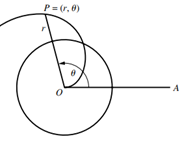
\includegraphics[height=0.4\linewidth]{7a}
		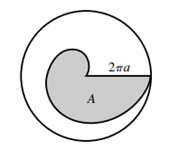
\includegraphics[height=0.4\linewidth]{7b}
%		\caption{\small\textit{\color{}.}}
%		\vspace*{-5pt}
	\end{figure}
	Theo quan điểm của toán học hiện đại, có lẽ thành tựu toán học vĩ đại nhất của Archimedes, và chắc chắn là một trong những kết quả thú vị nhất là công thức tính diện tích bao quanh bởi đường xoắn ốc đầu tiên (ứng với $0 \le \theta  \le 2\pi $). Ông đã viết: \textit{Diện tích giới hạn bởi đường xoắn ốc và đường thẳng ban đầu sau đúng một vòng quay bằng một phần ba diện tích hình tròn với bán kính là độ dài đoạn cuối chuyển động}. Điều này biểu thị theo công thức hiện đại là:  
	\begin{align*}
		S = \frac{1}{3}\pi {\left( {2\pi a} \right)^2}.
	\end{align*}
	Ngày nay, công thức trên dễ dàng được chứng minh nhờ phép tính tích phân. Archimedes đã sử dụng phương pháp vét kiệt: ông chia đường cong xoắn ốc thành nhiều phần, tính diện tích các phần và cộng chúng lại (hình dưới).
	\begin{figure}[H]
		\vspace*{-5pt}
		\centering
		\captionsetup{labelformat= empty, justification=centering}
		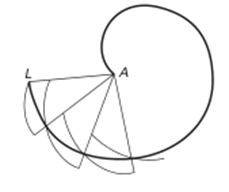
\includegraphics[width= 0.65\linewidth]{8}
%		\caption{\small\textit{\color{}.}}
		\vspace*{-10pt}
	\end{figure}
	Phương pháp vét kiệt được cho là của Eudoxus xứ Cnidos ($390-337$ trước CN), mặc dù Euclid và Archimedes sử dụng nó thường xuyên nhất và đem lại nhiều hiệu quả. Phương pháp này đóng một vai trò hàng đầu trong quyển XII của \textit{Cơ sở}, khi Eulid chứng minh rằng tỷ số diện tích các hình tròn bằng bình phương tỷ số đường kính và tỷ số thể tích các hình chóp có cùng chiều cao và có đáy tam giác bằng tỷ số diện tích đáy. Archimedes đã khai thác triệt để phương pháp vét kiệt để tìm diện tích các hình phẳng và thể tích hình giới hạn bởi các mặt cong. Cụm từ \textit{phương pháp vét kiệt} (method of exhaustion) lần đầu tiên được nhà toán học Dòng Tên Gregory St. Vincent dùng trong tác phẩm \textit{Opus Geometricum} ($1647$).
	\vskip 0.1cm 
	\textbf{\color{lichsutoanhoc}Cầu phương Parabola.} \textit{Cầu phương Parabola} gồm $24$ Mệnh đề ([$2$], trang $336-345$; [$3a$], trang $233-252$), trong đó Archimedes đã sử dụng phương pháp vét kiệt để tìm diện tích hình giới hạn bởi một parabola với một dây cung. Ông bắt đầu ``vét kiệt" diện tích parabola bằng cách nội tiếp trong nó một tam giác có đáy là dây cung và chiều cao bằng khoảng cách từ dây cung đến điểm trên parabola mà tại đó tiếp tuyến song song với dây cung. Hai cạnh còn lại của tam giác nội tiếp cho ta hai phần parabola mới. Diện tích mỗi tam giác nội tiếp cũng được tính tương tự (Hình dưới).
	\begin{figure}[H]
		\vspace*{-5pt}
		\centering
		\captionsetup{labelformat= empty, justification=centering}
		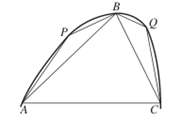
\includegraphics[height=0.35\linewidth]{9}
		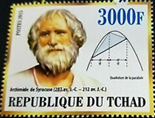
\includegraphics[height=0.35\linewidth]{9b}
		%		\caption{\small\textit{\color{}.}}
		\vspace*{-15pt}
	\end{figure}
	Như vậy, diện tích parabola bằng tổng vô hạn diện tích các tam giác và Archimedes đã chứng minh nó bằng $\frac{4}{3}$  diện tích tam giác ban đầu.   
	\vskip 0.1cm
	Lập luận của Archimedes là điển hình cho cách tiếp cận tổng quát của ông trong việc xác định diện tích hoặc thể tích bằng phương pháp vét kiệt.  Ký hiệu diện tích tam giác $CAB$ là $S$.  Từ tính chất của Parabola, Archimedes chứng minh được diện tích mỗi tam giác $PAB$  và $QBC$  bằng $\frac{1}{8}S$.  Các tam giác nhỏ hơn được xác định tương tự. Vậy, tổng diện tích các tam giác sau $n$  bước bằng
	\begin{align*}
		{S_n} &= S\left( {1 + \frac{1}{4} + \frac{1}{{{4^2}}} + ... + \frac{1}{{{4^n}}}} \right) \\
		&= S\left[ {\frac{4}{3} - \frac{1}{3}{{\left( {\frac{1}{4}} \right)}^n}} \right].
	\end{align*}
	Theo lập luận hiện đại, diện tích của phần chắn bởi parabola và cát tuyến của nó chính là giới hạn của $S_n$  khi $n \to \infty$,  tức là  $\mathop {\lim }\limits_{n \to \infty } {S_n} = \frac{4}{3}S.$
	\vskip 0.1cm
	Tuy nhiên, vì chưa có khái niệm giới hạn, Archimedes đã chứng minh bằng cách \textit{lập luận vô lý rút gọn kép} (a double reductio ad absurdum argument): Nếu các đa giác vét kiệt parabola, thì diện tích của parabola không thể nhỏ hơn, cũng không thể lớn hơn $\frac{4}{3}S.$
	\vskip 0.1cm  
	Trong Lời nói đầu của \textit{Phương pháp} (Method, [$3b$]), Archimedes viết: \textit{Tôi cho rằng một số các thế hệ hiện tại cũng như tương lai, phương pháp [vét kiệt] được giải thích ở đây, sẽ được kích hoạt để tìm ra những định lý khác mà chúng ta chưa rõ}. Thật không may, sau Archimedes, toán học Hy Lạp đã đi theo hướng khác.  Chỉ sau $18$ thế kỷ, phương pháp vét kiệt mới được hoàn chỉnh thành phép tính vi phân và tích phân nhờ Newton và Leibniz. 
	\vskip 0.1cm
	Archimedes chết, như ông đã sống, chìm đắm trong những suy tư và chiêm nghiệm toán học của mình. 
	\vskip 0.1cm
	\textbf{\color{lichsutoanhoc}Kết luận.} Trong một bài viết, không thể nói đầy đủ về Archimedes, thậm chí chỉ về toán học của ông. Thật là khiếm khuyết khi bài viết không đề cập đến các công trình của Archimedes về thủy tĩnh học, về cân bằng,\ldots\, Hy vọng nó sẽ được đề cập trong một bài khác. 
	\vskip 0.1cm
	Bạn đọc có thể tìm hiểu thêm về Archimedes qua các tài liệu tham khảo. Để phần nào hình dung thêm các đóng góp và phát triển của ông trong toán học Hy Lạp, có thể tham chiếu thêm [$11$].
	\vskip 0.1cm
	Không ai khác, chính là hình Archimedes đã được in trên tấm huy chương danh giá nhất của giới toán học:
	\vskip 0.1cm
	Huy chương Fields được thiết kế bằng vàng, in hình đầu của nhà toán học Archimedes với dòng trích dẫn lời của ông: \textit{Transire suum pectus mundoque potiri (Hãy vươn ra ngoài giới hạn của bản thân và làm chủ thế giới}, hay \textit{Vượt lên chính mình và thấu hiểu thế giới).}
		\begin{figure}[H]
		\vspace*{5pt}
		\centering
		\captionsetup{labelformat= empty, justification=centering}
		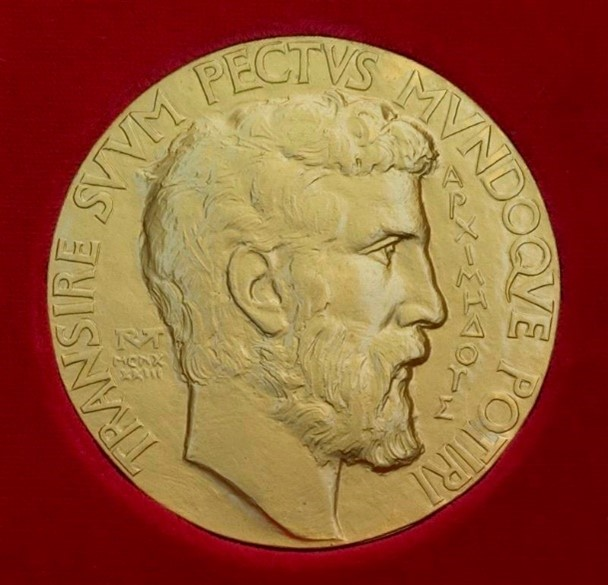
\includegraphics[width= 1\linewidth]{10}
		%		\caption{\small\textit{\color{}.}}
		\vspace*{-10pt}
	\end{figure}
	\textbf{\color{lichsutoanhoc}Lời cảm ơn.} Tác giả cảm ơn Thạc sĩ Nguyễn Hoàng Vũ đã cung cấp Tài liệu [$2$].
	\vskip 0.1cm
	\textbf{\color{lichsutoanhoc}Tài liệu tham khảo chính}
	\vskip 0.1cm
	[$1$] David M. Burton, \textit{The History of Mathematics, An Introduction}, Seventh Edition, McGraw--Hill, $2011$. Ch. $4$: The Alexandrian School: Archimedes, pp. $193-206$.
	\vskip 0.1cm
	[$2$] E. J. Dijksterhuis, \textit{Archimedes}, Princeton University Press, Princeton, New Jersey, USA, $1987$. 
	\vskip 0.1cm
	[$3a$] Thomas L. Heath, \textit{The Works of Archimedes}, Cambridge: At the University Press, $1897$.
	\vskip 0.1cm
	[$3b$] Thomas L. Heath, \textit{The Method of Archimedes}, Recently discovered by Heiberg, A supplement to \textit{The Works of Archimedes},  Cambridge: At the University Press, $1912$.
	\vskip 0.1cm
	[$3c$] Thomas L. Heath, \textit{Archimedes}, London, Society for Promoting Christian Knowledge, $1920$.
	\vskip 0.1cm
	[$4$] Thomas L. Heath, \textit{A History of Greek Mathematics}, Oxford at the Clarendon Press, $1921$, Volume 1I: Archimedes, pp. $16-109$.   
	\vskip 0.1cm
	[$5$] Stephen Hawking, \textit{God Created the Integers, The mathematical Breakthroughs that changed History}, Running Press, London, $2007$, \textit{Archimedes}, pp. $119-240$.
	\vskip 0.1cm   
	[$6$] Uta C. Merzbach and Carl B. Boyer, \textit{A
	History of Mathematics}, $3$th Edition, John Wiley \& Sons, $2011$, Ch. $6$: Archimedes of Syracuse, pp. $109-126$.
	\vskip 0.1cm
	[$7$] Victor J. Katz, \textit{A History of Mathematics, An Introduction}, Third Edition, Addison--Wesley, $2008$. Chapter $4$: \textit{Archimedes and Apollonius}, pp. $94-111$.
	\vskip 0.1cm
	[$8$] Lê Thanh Quang, \textit{Kể chuyện các nhà toán học}, Nhà xuất bản Lao động, $2016$, $Archimedes$, trang $5-16$.
	\vskip 0.1cm
	\textbf{\color{lichsutoanhoc}Tài liệu trích dẫn}
	\vskip 0.1cm
	[$9$] Phạm Triều Dương, \textit{Những câu nói cuối cùng huyền thoại của Archimedes}, Tạp chí Pi, Tập $7$, số $5$, trang $8-10$.
	\vskip 0.1cm
	[$10$] Đỗ Trọng Đạt, Phó Đức Tài, \textit{Phương pháp Archimedes tính các hình khối quen thuộc}, Tạp chí Pi, Tập $2$, số $3$, trang $34-36$.
	\vskip 0.1cm
	[$11$] Tạ Duy Phượng, \textit{Các nhà toán học Hy Lạp}, Tạp chí Pi, Tập $6$, số $4$, trang $46-50$; số $5$, trang $45-53$; số $9$, trang $44-51$; số $10$, trang $56-59$; số $11$, trang $51-55$; Tập $7$, số $4$, trang $54-60$; số $5$, trang $52-60$.
	[$12$] Tạ Duy Phượng, Đoàn Thị Lệ, Cung Thị Kim Thành, Mai Văn Thu, Nguyễn Hoàng Vũ, \textit{Tính số Pi: Xưa và Nay. Phần I: Tính số Pi: Xưa}, Tạp chí Pi, Tập $7$, số $3$, trang $44-51$.
	\vskip 0.1cm
	[$13$] Hà Huy Thái, \textit{Archimedes và số  $\pi$} Tạp chí Pi, Tập $3$, số $10$, trang $37-41$.
\end{multicols}